\chapter{Implementation} \label{cha:Implementation}
The design considerations and their reflecting implementations are detailed in this chapter.

\section{Path simulation}
To simulate a path following a Brownian motion, as in (\ref{eqn:BlackScholesSDE}) and later in (\ref{eqn:Stilde1})-(\ref{eqn:StjFinal}), we must generate and consume random normal variables $Z_i$. The main focus of this project is to improve efficiency and speed when calculating Greeks and so we are not concerned with the performance when generating random variables. The basics of random number generation are discussed in sections \ref{sec:prng} through \ref{sec:ScrambledSobol}. There exist many libraries for random number generation and we choose to use cuRAND \cite{curand} due to it being part of the CUDA toolkit.

To utilise the highly parallel nature of the GPU, each thread will be responsible for the simulation of one path. This requires each thread to have access to it's own distinct set of random variables and a place to store the results from path simulation. The loading and storing of these values is of key importance during the simulation. Due to the number of random variables required we store the arrays in \textit{global memory} which is a slower, but larger, type of memory available in the CUDA architecture. The access pattern to global memory can have a huge impact on the performance of a kernel. Here, we detail the concept of \textit{coalesced memory accesses}. As discussed in \ref{sec:cudaarch} threads are are arranged into groups of 32 known as a \textit{warp}. Accesses to global memory in CUDA are coalesced such that 32-, 64- and 128-byte accesses are loaded in a single transaction, shown in Figure \ref{fig:coalescedaccess}. In our implementation, each block contains $64$ threads, so at each timestep two warps will load their random variables in just two memory transactions.

\begin{figure}[h]
    \centering
    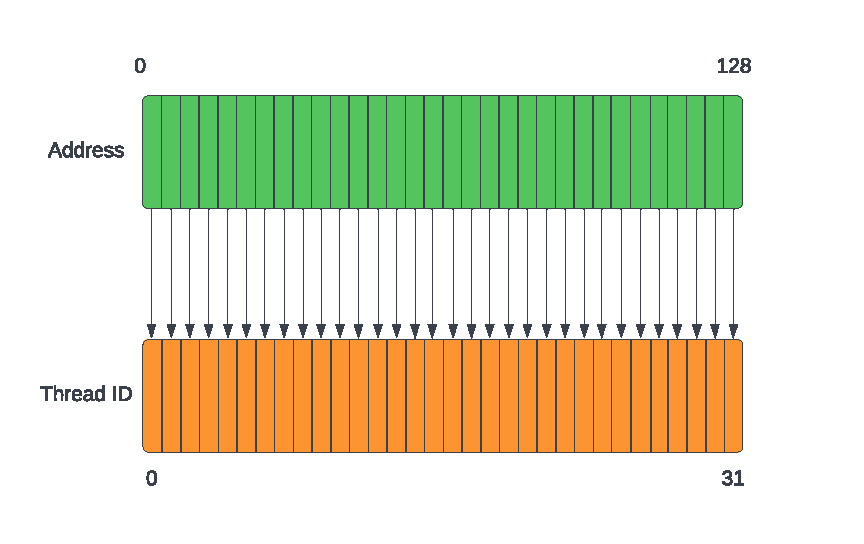
\includegraphics[width=0.8\textwidth]{figures/coalesced access.pdf}
    \caption{Coalesced memory access where a warp of 32 threads loads 128-bytes in a single transaction. Inspired by: https://cvw.cac.cornell.edu/gpu/coalesced}
    \label{fig:coalescedaccess}
\end{figure}

Therefore it is extremely important that we load random variables in a way that minimises the number of transactions (due to the much slower global memory). If we were to arrange the accesses such that each thread were to load $N$ contiguous random variables from memory during path simulation, at each step we would have to sequentially perform a separate memory transaction for each thread. This can incur costs of a lot more than 10x when compared to coalesced accesses. As such, we access random variables such that a single transaction satisfies a whole warp.


To perform path generation, we use two types of random number generator from cuRAND: \texttt{CURAND_RNG_PSEUDO_DEFAULT} and \texttt{CURAND_RNG_QUASI_SCRAMBLED_SOBOL32}. Due to the nature of low-discrepancy sequences we must specify a dimension for the Sobol' generator, we use the number of timesteps in a simulation. We have to pay close attention to the dimensions when using the random variables from the quasi generator as the simulation of each timestep must be independent from each other, thus we must use a random variable from a different dimension. By default, the cuRAND Sobol' generator will output $N/d$ numbers from dimension $1$, followed by $N/d$ from dimension $2$ when generating $N$ variables in $d$ dimensions. The ordering of dimensions is not well spatially-located so we choose to transform the ordering so that coalesced memory access with a smaller stride are possible. Algorithm \ref{alg:QuasiRandomNumbersTransformation} demonstrates this transformation.

\begin{algorithm}[hbt!]
\caption{Transformation of quasi-random variables from $N*\text{PATHS}/d$ of each dimension to BLOCK_SIZE of each dimension repeated, where $N$ is the number of timesteps.}\label{alg:QuasiRandomNumbersTransformation}
\begin{algorithmic}[1]
\State $\text{d_z[PATHS*N]}$ \Comment{Output array} 
\State $\text{temp_z[PATHS*N]}$ \Comment{Input array of random numbers}
\State $\text{desired_idx} \gets \text{threadIdx.x} + \text{N} * \text{blockIdx.x} * \text{blockDim.x}$
\State $\text{temp_idx} \gets \text{threadIdx.x} + \text{blockIdx.x} * \text{blockDim.x}$
\For{$i \gets 0..N-1$}
    \State $\text{d_z[desired_idx]} \gets \text{temp_z[temp_idx]}$
    \State $\text{desired_idx} \gets \text{desired_idx} + \text{blockDim.x}$
    \State $\text{temp_idx} \gets \text{temp_idx} + \text{PATHS}$
\EndFor
\end{algorithmic}
\end{algorithm}

Shown in in Figure \ref{fig:QuasiVariableTransformation} is the input and output ordering of random variables. We see that $B$ variables, where $B$ is BLOCK\_DIM, are taken from each dimension and placed next to each other. This process is repeated such that we have PATHS sets of random numbers from dimension $1$ to $d$. One set will be used by one block such that the BLOCK\_SIZE threads in that block simulate a single path each (one timestep uses one of the dimensions), with the random variable accesses being coalesced.

\begin{figure}[h]
    \centering
    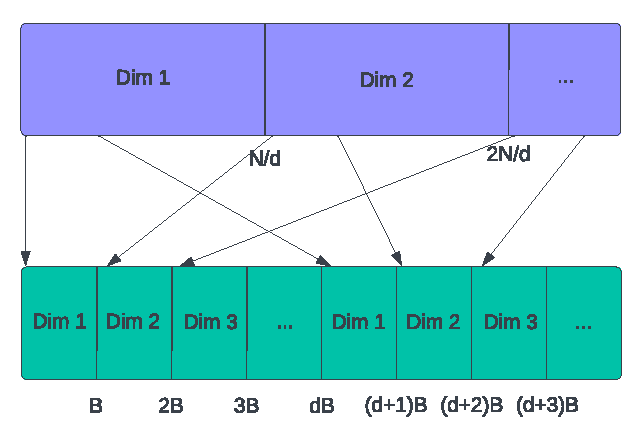
\includegraphics[width=0.7\textwidth]{figures/quasi ordering transform.pdf}
    \caption{Transformation of cuRAND Sobol' numbers from input (top) to output (bottom) ordering.}
    \label{fig:QuasiVariableTransformation}
\end{figure}

In order to reduce the memory footprint and number of accesses, the results of path simulation are not stored for standard MC and standard QMC and required results are calculated on-the-fly during path simulation. This decision also reinforces the decision to encapsulate simulation inside of each product - discussed in \ref{sec:Products}. This allows us to store values required for calculation of the Greeks (such as $S_A$) whilst simulating the path, and use them in the later steps. The basic steps are outlined in Algorithm \ref{alg:PathSimulation}. The separation of $S$ and $\widetilde{S}$ is necessary so that we are able to calculate the Greeks estimates as per section \ref{sec:qmc-cpwmethod}. For QMC with Brownian bridge construction (see \ref{sec:BBConstructionResults} for futher description) we must store the intermediate Brownian bridge results to consume them for path generation afterwards.

\begin{algorithm}[hbt!]
\caption{Per-thread path simulation where $N$ is the number of simulated timesteps with $dt = 1/N$}\label{alg:PathSimulation}
\begin{algorithmic}[1]
\State $S \gets S_0$
\State $Z \gets \text{RandomNormals[ind]}$
\State $W_1 \gets sqrt(dt) * Z$
\State $\widetilde{W}_1 \gets W_1$
\For{$i \gets 1..N$}
    \State $\text{ind} \gets \text{ind} + \text{blockDim.x}$ \Comment{Coalesced reads, when blockDim.x is a multiple of 32}
    \State $Z \gets \text{RandomNormals[ind]}$
    \State $\widetilde{W}_i \gets \widetilde{W}_i + sqrt(dt) * Z$
    \State $\widetilde{S} \gets S_0 * \exp{(\omega * (n-1)*dt + \sigma * (\widetilde{W} - W_1))}$
    \State $S \gets \widetilde{S} * \exp{(\omega * dt + \sigma * W_1)}$
\EndFor
\end{algorithmic}
\end{algorithm}

\section{Products} \label{sec:Products}
It is required to calculate the prices and sensitivities of a variety of options and the functions to do so typically vary between different option types. However, the overall process is the same for pricing any derivative, namely: simulate paths of the underlying asset, followed by calculating the prices and Greeks given the simulated path. These two requirements are that of any option and as such we combine them into a \textit{product}. In this paper we focus on three types of exotic option: arithmetic Asian, binary Asian and lookback. For derivations of the Greek estimates as in \ref{sec:qmc-cpwmethod} see section \ref{sec:GreeksCalculation}. Each of these products implements its own path simulation and Greeks calculation method.

Inheritance and virtual functions are widely-used in standard C++ and similar programming languages, however there are many more restrictions with CUDA. Due to having separate address spaces, copying objects with virtual functions from host memory to device memory can be tricky. To avoid unnecessary complexity, we avoid the use of inheritance directly in kernels (on device) and use them only to aid readability and development. To avoid inheritance directly, we make use of templating in C++. That is, kernels which are used for multiple option types are templated so that at compile time distinct versions of the kernel are generated for each option. From this we obtain the same benefits from inheritance such as minimal repetition of code, without having to copy objects with virtual function tables across address spaces or perform any casts. 

Each thread instantiates its own local copy of the product which has member fields for values such as the underlying's price at the current timestep, running averages, and index to the current random variable. The \textit{SimulatePath} method is called and that thread performs a single simulation for the product, calculating any intermediate values such as the average underlying price or the inner sum of the vega estimate. The final call is to the \textit{CalculatePayoffs} function which calculates the price of the option and Greeks, then places these values back into the global struct of arrays of results.

\section{Antithetic variables}
As a variance reduction technique we have used antithetic variables as described in \ref{sec:antitheticvariables}. Using the already generated random normal variables for the standard MC simulation, we take their complement and simulate a second path from which another set of estimates are calculated. The estimates from the standard and antithetic paths can then be combined to produce the variance reduced final estimate. Adding antithetic variables requires minimal storage on device as we only need to add fields to our products struct that represent the antithetic counterpart to the standard MC values such as $\widetilde{S}(t_j)$.

\section{Brownian bridge construction} \label{sec:BBConstructionResults}
For QMC, we have implemented Brownian bridge construction as a variance reduction method. As shown in Algorithm \ref{alg:PathSimulation} we generate the Brownian motion $\widetilde{W}_i$ from left to right (i.e. from $i=1\dots,d$). However, we may choose to generate the $\widetilde{W}_i$ in any order as long as we sample from the correct conditional distribution given the values already generated. Conditioning a Brownian motion on its endpoints produces a \textit{Brownian bridge} \cite{glasserman2004monte}. The basic idea is that we generate the final value $\widetilde{W}_d$, then continue to fill in each intermediate value: $\widetilde{W}_{d/2}$, then $\widetilde{W}_{d/4}$ and $\widetilde{W}_{3d/4}$ etc, until all values are calculated. For further explanation of how the conditional mean and variance are derived, the reader is referred to section 3.1 of \cite{glasserman2004monte}.

Our implementation does not construct the path directly using a Brownian bridge, but rather uses the bridge to calculate the increments in the path. This allows us to construct $\widetilde{W}$ simply by iterating through the output of the Brownian bridge construction and adding it to the previous value. Algorithm \ref{alg:BrownianBridgeConstruction} demonstrates the process of constructing the Brownian bridge increments.

\begin{algorithm}[hbt!]
\caption{Construction of Brownian bridge increments where the number of timesteps is equal to $2^m$. \textit{idx_zero} is passed to each thread as the first index into the global path array.}\label{alg:BrownianBridgeConstruction}
\begin{algorithmic}[1]
\State $\text{path[idx_zero]} \gets \text{d_z[idx]}$ \Comment{Put first random variable (representing terminal value) in path}
\For{$k \gets 1..m$}
    \State $i \gets 2^k - 1$
    \For{$j \gets 2^{k-1}-1..0$}
        \State $\text{idx} \gets \text{idx} + \text{blockDim.x}$ \Comment{Access next random variable}
        \State $z = \text{d_z[idx]}$
        \State $a \gets 0.5 * \text{path[idx_zero} + j * \text{blockDim.x]}$
        \State $b \gets \sqrt{1 / 2^{k+1}}$
        \State $\text{path[idx_zero} + i * \text{blockDim.x]} \gets a - b * z$
        \State $i \gets i - 1$
        \State $\text{path[idx_zero} + i * \text{blockDim.x]} \gets a + b * z$
        \State $i \gets i - 1$
    \EndFor
\EndFor
\end{algorithmic}
\end{algorithm}

Brownian bridge construction gives finer control over the overall structure of the simulated path as opposed to the standard recursion technique: we use only one random variable to generate the terminal value and then continue to add more and more detail to the rest of the path. Furthermore, when using Sobol' sequences, the first random variables are particularly well distributed leading to the terminal values also being well distributed. This is due to the fact that the initial coordinates of a Sobol' sequence have superior uniformity to that of higher-indexed coordinates \cite{glasserman2004monte}. As the terminal value is often more important than other values in the path this can lead to less error in the estimates produced by Brownian bridge construction with Sobol' sequences. An example of how the path is generated as more points are sampled can be seen in Figure \ref{fig:BrownianBridgePlots}.

The main downside with performing Brownian bridge construction rather than the standard approach is that we need to store the generated path to later consume to simulate the stock price in the variable separated form as per \ref{sec:VariableSeparationPathSimulation}. This means we not only use more global memory on device but will also have a slower kernel runtime due to the increase in memory accesses. However, with this trade-off we expect to achieve a much smaller error in our estimates.

\begin{figure}[h]
    \centering
    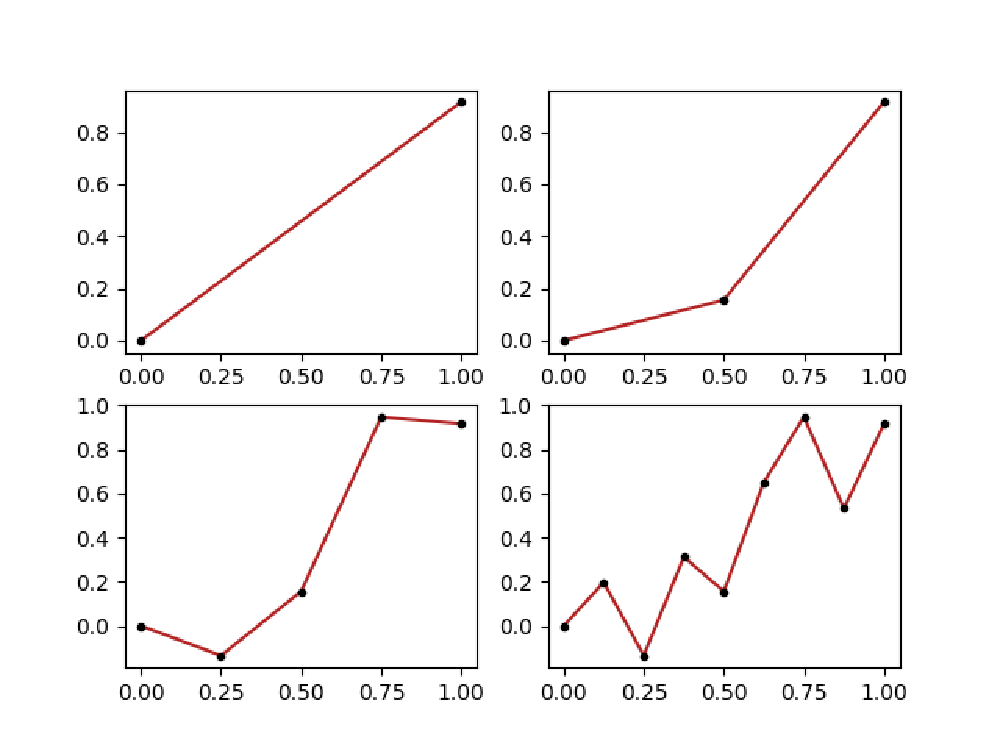
\includegraphics[width=0.8\textwidth]{figures/bb construction.pdf}
    \caption{Brownian bridge construction after $1$, $2$, $4$ and $8$ points have been sampled conditional on the previous values generated.}
    \label{fig:BrownianBridgePlots}
\end{figure}

\section{Greeks calculation} \label{sec:GreeksCalculation}
The step of calculating Greeks is actually quite straightforward. Once we have simulated the path and saved the required values we simply need to evaluate the estimates and store them. Below we list the derived Greeks that are used to calculate estimates as per \cite{ZhangConditionalQuasiMonteCarloMethod} following on from the example in \ref{sec:BaDeltaExample}.

\subsection{Binary Asian Greeks}
As we have already shown the full derivation for the delta, we continue with the estimates for gamma and vega.

\begin{equation*}
\begin{aligned}
    gamma: \frac{{\partial}^2 G}{\partial {S(0)}^2} &= \frac{e^{-rT}}{{S(0)}^2\sigma \sqrt{t_1}}\phi(\psi_d)\left(\frac{\psi_d}{\sigma \sqrt{t_1}} - 1\right). \\[10pt]
\end{aligned}
\end{equation*}

\begin{equation*}
\begin{aligned}
    vega: \frac{{\partial}^2 G}{\partial \sigma} &= e^{-rT}\phi(\psi_d) \left[ \frac{1}{d\sigma \sqrt{t_1}\widetilde{S}_A} \sum_{j=1}^d{\widetilde{S}(t_j) (\widetilde{B}(t_j - t_1) - \sigma(t_j - t_1))} + \frac{\psi_d}{\sigma} - \sqrt{t_1} \right]. \\[10pt]
\end{aligned}
\end{equation*}

Note that the sum inside of the vega calculation is an example of one of the values that is calculated on-the-fly during the path simulation, allowing us to disregard storing the path for standard MC and QMC and storing single precision values only.

\subsection{Arithmetic Asian Greeks}
By taking the conditional expectation we obtain the smoothed payoff

\begin{equation*}
    G(\theta, \boldsymbol{z}) = e^{r(t_1 - T)} \widetilde{S}_A \left[1 - \Phi(\psi_d - \sigma \sqrt{t_1} \right] - e^{-rT}K\left[ 1 - \Phi(\psi_d) \right]
\end{equation*}

We can now differentiate with respect to our parameters of interest to obtain the following estimates.

\begin{equation*}
\begin{aligned}
    delta: \frac{\partial G}{\partial {S(0)}} &= e^{r(t_1 - T)} \frac{\widetilde{S}_A}{S(0)}\left[1 - \Phi(\psi_d - \sigma \sqrt{t_1}) \right]. \\[10pt]
\end{aligned}
\end{equation*}

\begin{equation*}
\begin{aligned}
    gamma: \frac{{\partial}^2 G}{\partial {S(0)}^2} &= \frac{Ke^{-rT}}{{S(0)}^2\sigma\sqrt{t_1}} \phi(\psi_d). \\[10pt]
\end{aligned}
\end{equation*}

\begin{equation*}
\begin{aligned}
    vega: \frac{{\partial} G}{\partial \sigma} &= e^{r(t_1 - T)} \left[1 - \Phi(\psi_d - \sigma \sqrt{t_1}) \right] \frac{1}{d}\sum_{j=1}^d{\widetilde{S}(t_j) (\widetilde{B}(t_j - t_1) - \sigma(t_j - t_1))} + Ke^{-rT}\phi(\psi_d)\sqrt{t_1}. \\[10pt]
\end{aligned}
\end{equation*}

\subsection{Lookback Greeks}
Again, we take the conditional expectation to obtain the smoothed payoff

\begin{equation*}
    G(\theta, \boldsymbol{z}) = e^{r(t_1 - T)} \widetilde{S}_{max} \left[1 - \Phi(\psi_d - \sigma \sqrt{t_1} \right] - e^{-rT}K\left[ 1 - \Phi(\psi_d) \right],
\end{equation*}

where $\widetilde{S}_{max}$ is the maximum value of $\widetilde{S}(t_j)$ for $j = 1,\dots,d$, and $\psi_d = (\ln{K} - \ln{\widetilde{S}_{max}} - \omega t_1) / \sigma \sqrt{t_1}$. By taking differentiation with respect to our parameters we obtain the estimates

\begin{equation*}
\begin{aligned}
    delta: \frac{\partial G}{\partial {S(0)}} &= e^{r(t_1 - T)} \frac{\widetilde{S}_{max}}{S(0)}\left[1 - \Phi(\psi_d - \sigma \sqrt{t_1}) \right]. \\[10pt]
\end{aligned}
\end{equation*}

\begin{equation*}
\begin{aligned}
    gamma: \frac{{\partial}^2 G}{\partial {S(0)}^2} &= \frac{Ke^{-rT}}{{S(0)}^2\sigma\sqrt{t_1}} \phi(\psi_d). \\[10pt]
\end{aligned}
\end{equation*}

\begin{equation*}
\begin{aligned}
    vega: \frac{{\partial} G}{\partial \sigma} &= e^{r(t_1 - T)} \left[1 - \Phi(\psi_d - \sigma \sqrt{t_1}) \right] \frac{1}{d}\sum_{j=1}^d{\widetilde{S}(t_j) (\widetilde{B}(t_j - t_1) - \sigma(t_j - t_1)) \boldsymbol{1}\{\widetilde{S}(t_j) = \widetilde{S}_{max}\}}\\ 
    &\quad + Ke^{-rT}\phi(\psi_d)\sqrt{t_1}. \\[10pt]
\end{aligned}
\end{equation*}

\section{Likelihood Ratio estimates}
As a baseline for the error in the Greek estimates, we implement the LR method through Monte Carlo simulation. Taking the ideas in \ref{sec:LikelihoodRatioMethod} we apply LR to our set of options. The expression given in (\ref{eqn:LRUnbiasedEstimate}) shows that

\begin{equation*}
    f(X) \frac{g^\prime_\theta(X)}{g_\theta(X)},
\end{equation*}

is an unbiased estimator of the derivative of $E[Y]$ with respect to parameter $\theta$. The expression $g^\prime_\theta(X)/g_\theta(X)$ is commonly referred to as the \textit{score}. Calculating Greeks using LR simplifies to calculating the product of the discounted payoff and the relevant score for the Greek. 

Below are listed the scores for the Greeks of each of the three options we are concerned with.

\begin{equation*}
\begin{aligned}
    delta: \frac{Z_1}{S(0)\sigma\sqrt{t_1}}. \\[10pt]
\end{aligned}
\end{equation*}
\begin{equation*}
\begin{aligned}
    gamma: \frac{Z_1^2 - 1}{{S(0)}^2 \sigma^2 t_1} - \frac{Z_1}{{S(0)}^2 \sigma \sqrt{t_1}}. \\[10pt]
\end{aligned}
\end{equation*}
\begin{equation*}
\begin{aligned}
    vega: \sum_{j=1}^d{\frac{Z_j^2 - 1}{\sigma} - Z_j\sqrt{t_1}}. \\[10pt]
\end{aligned}
\end{equation*}

Note that the scores for the three options are equal and the difference between the estimates is simply the form of the payoff.

\section{CPU implementation}
To demonstrate the superior speed when using GPUs we implement a naive, sequential Monte Carlo simulation with the same form of estimates from the aforementioned sections. The implementation has the general form shown in Algorithm \ref{alg:EstimateExpectedPayoff}. The random normal variables generated for use in the GPU simulation are reused by the CPU simulation, in which a single thread performs \textit{NPATH} simulations of $N$ timesteps each. After each path simulation the estimates are calculated and stored in the results struct in the same way that a single GPU thread does.

\chapter{Results} \label{cha:Results}
To demonstrate the effectiveness of the QMC-CPW method from section \ref{sec:qmc-cpwmethod} we run many simulations on the GPU and calculate the variance reduction factors (VRFs) for multiple methods. Using the Likelihood Ratio estimate as the baseline for variance, the VRF for a method is calculated as 

\begin{equation*}
    \frac{\sigma^2_0}{\sigma^2},
\end{equation*}

where $\sigma^2_0$ is the variance in the LR estimate for the Greek. For all methods the estimates for the Greeks are calculated over $P$ number of paths of $N$ timesteps, such that the estimate from a single path is given as

\begin{equation*}
    C^{(\ell)} = {F(\theta,\boldsymbol{z}_\ell}),
\end{equation*}

where $\boldsymbol{z}_\ell$ is a vector of $N$ normal random variables and $F(\theta, x)$ is the underlying function we wish to estimate (e.g. the delta estimate for an arithmetic Asian option). To calculate the error in the estimate we perform $L$ independent runs of the simulation with $P$ fixed such that the final estimate is given as

\begin{equation*}
    C = \frac{1}{L} \sum_{\ell=1}^{L} C_P^{(\ell)},
\end{equation*}

where $C_P^{(\ell)}$ is the estimate from the $\ell$th run over $P$ paths. Finally, the error in the estimate is calculated as follows:

\begin{equation*}
    \sigma = \sqrt{\frac{1}{L} \sum_{\ell=1}^{L} {(C - C_P^{(\ell)})}^2}.
\end{equation*}

For delta, gamma and vega estimation we compare four methods: standard Monte Carlo with CPW estimates (MC-CPW), Monte Carlo with antithetic variables and CPW estimates (MC+AV-CPW), Quasi-Monte Carlo with CPW estimates (QMC-CPW), and finally Quasi-Monte Carlo with Brownian bridge construction and CPW estimates (QMC+BB-CPW). Following a similar style as in \cite{ZhangConditionalQuasiMonteCarloMethod} we perform the simulations over a range of strike prices $K=90,100,110$, and two values for the number of discrete time steps $d=64,256$. We denote the option as "in the money" at $K=90$, "at the money" at $K=100$ and "out the money" at $K=110$. The number of paths, initial stock price, volatility, and risk-free interest rate are all constant and equal for each option type with $P = 2^{15}$,  $S(0) = 100$, $\sigma = 0.2$, and $r = 0.1$. The expiration date for each option $T = 1.0$, or one year. We perform $L=500$ independent runs for all methods. The VRFs for arithmetic, binary and lookback options are presented in tables \ref{tbl:vrfs-arithmetic}-\ref{tbl:vrfs-lookback} respectively. Later we discuss the behaviour of the error in Greek estimates as we increase the number of path simulations per independent run. Information about the \textit{Tesla T4} GPU and the specifications of the CUDA toolkit that was used to collect the results can be found in Appendix \ref{app:gpu-cuda-specs}.

We can make the following observations from the experimental results:

\begin{itemize}
    \item The QMC+BB-CPW method is the most accurate in almost all cases. This is due to the combination of the CPW method which smooths the integrand, allowing for QMC method to work more efficiently, and the Brownian bridge construction which further reduces variance through the methods described in section \ref{sec:BBConstructionResults}.
    \item For the arithmetic Asian option we see QMC+BB-CPW as the best method in all experiments, with VRFs in the hundreds of thousands, and in many cases more than $10$x accurate in comparison to QMC-CPW and MC+AV-CPW. When looking at the VRFs for gamma estimates of the arithmetic Asian option (Table \ref{tbl:vrfs-arithmetic}), MC+AV-CPW outperforms QMC-CPW and this could be due to MV+AV-CPW effectively simulating twice as many paths (standard + antithetic paths) which of course helps to reduce the variance. However, this is not the case for the delta and vega estimates which is interesting to note.
    \item Strike price does affect the performance of many experiments, particularly for the delta and gamma estimates, in which we see an increase in the strike leading to a decrease in VRF.
    \item We discuss dimensionality later, but it also has an effect on the accuracy and becomes more apparent for QMC methods.
\end{itemize}

\begin{table}[!h]
\centering
$\begin{array}{ c c c c c c c c } 
 \hline
 \text{Greeks} & K & d & \text{LR+MC} & \text{MC-CPW} & \text{MC+AV-CPW} & \text{QMC-CPW} & \text{QMC+BB-CPW} \\
 \hline
 \text{delta} & 90  & 64  & 1 & 623     & 3{,}209 & 5,784    & \boldsymbol{154{,}860} \\ 
              &     & 256 & 1 & 2{,}159 & 9{,}527 & 11{,}976 & \boldsymbol{106{,}806} \\
              & 100 & 64  & 1 & 106     & 963     & 903      & \boldsymbol{52{,}689} \\
              &     & 256 & 1 & 353     & 2{,}702 & 1{,}735  & \boldsymbol{34{,}478} \\
              & 110 & 64  & 1 & 35      & 172     & 207      & \boldsymbol{13{,}226} \\
              &     & 256 & 1 & 103     & 423     & 445      & \boldsymbol{7{,}645} \\
 \\
 \text{vega} & 90  & 64  & 1 & 471     & 1{,}566 & 14,603   & \boldsymbol{442{,}513} \\ 
             &     & 256 & 1 & 1{,}595 & 5{,}424 & 30{,}894 & \boldsymbol{340{,}858} \\
             & 100 & 64  & 1 & 294     & 759     & 7{,}770  & \boldsymbol{376{,}285} \\
             &     & 256 & 1 & 967     & 2{,}540 & 18{,}162 & \boldsymbol{633{,}051} \\
             & 110 & 64  & 1 & 113     & 289     & 3{,}195  & \boldsymbol{119{,}816} \\
             &     & 256 & 1 & 330     & 917     & 6{,}701  & \boldsymbol{294{,}813} \\
 \\
 \text{gamma} & 90  & 64  & 1 & 20{,}393  & 49{,}141  & 28{,}067  & \boldsymbol{271{,}351} \\ 
              &     & 256 & 1 & 108{,}667 & 275{,}370 & 134{,}644 & \boldsymbol{487{,}940} \\
              & 100 & 64  & 1 & 3{,}814   & 9{,}433   & 5{,}427   & \boldsymbol{75{,}020} \\
              &     & 256 & 1 & 20{,}967  & 49{,}834  & 21{,}116  & \boldsymbol{72{,}558} \\
              & 110 & 64  & 1 & 1{,}101   & 2{,}468   & 1{,}477   & \boldsymbol{23{,}085} \\
              &     & 256 & 1 & 5{,}977   & 13{,}770  & 6{,}147   & \boldsymbol{25{,}695} \\
 \hline
\end{array}$
\caption{VRFs for arithmetic Asian option on GPU with $2^{15}$ paths. $S(0) = 100$, $\sigma = 0.2$, $r = 0.1$ and $T = 1$.}
\label{tbl:vrfs-arithmetic}
\end{table}

\begin{itemize}
    \item For delta and vega estimates of the binary Asian option (Table \ref{tbl:vrfs-binary}) we see QMC+BB-CPW outperforming all other methods and taking advantage of the increased smoothness of the integrand.
    \item We see little or no improvement of QMC-CPW over MC-CPW for all estimates of the binary option which could be an indication of the limitations of QMC in high dimensions.
    \item We also see this in the gamma estimates for the binary Asian option, where even QMC+BB-CPW is outperformed by MC+AV-CPW for all of the experiments with $256$ timesteps. A technique to reduce the effective dimension of the problem such as Principle Component Analysis (PCA) would likely remove these differences and result in a substantial decrease in error for the QMC methods.
    \item The binary Asian option results in some of the smallest VRFs for all Greek estimates especially for the delta and gamma.
    \item Again, we see the strike price having a large impact on the VRFs. For example the delta estimate with $K=90$ over $256$ timesteps in Table \ref{tbl:vrfs-binary} is $714$ and decreases to $150$ for $K=110$.
\end{itemize}

\begin{table}[!h]
\centering
$\begin{array}{ c c c c c c c c } 
 \hline
 \text{Greeks} & K & d & \text{LR+MC} & \text{MC-CPW} & \text{MC+AV-CPW} & \text{QMC-CPW} & \text{QMC+BB-CPW} \\
 \hline
 \text{delta} & 90  & 64  & 1 & 109 & 247 & 150 & \boldsymbol{1{,}447} \\ 
              &     & 256 & 1 & 159 & 389 & 197 & \boldsymbol{714} \\
              & 100 & 64  & 1 & 43  & 123 & 58  & \boldsymbol{830} \\
              &     & 256 & 1 & 64  & 150 & 64  & \boldsymbol{221} \\
              & 110 & 64  & 1 & 23  & 69  & 32  & \boldsymbol{497} \\
              &     & 256 & 1 & 35  & 89  & 36  & \boldsymbol{150} \\
 \\
 \text{vega} & 90  & 64  & 1 & 326     & 733     & 447     & \boldsymbol{4{,}227} \\ 
             &     & 256 & 1 & 481     & 1{,}168 & 593     & \boldsymbol{2{,}114} \\
             & 100 & 64  & 1 & 771     & 2{,}078 & 1{,}176 & \boldsymbol{12{,}571} \\
             &     & 256 & 1 & 1{,}419 & 3{,}405 & 1{,}502 & \boldsymbol{5{,}111} \\
             & 110 & 64  & 1 & 839     & 1{,}965 & 1{,}167 & \boldsymbol{9{,}232} \\
             &     & 256 & 1 & 1{,}976 & 4{,}617 & 1{,}950 & \boldsymbol{7{,}803} \\
 \\
 \text{gamma} & 90  & 64  & 1 & 363 & 713                  & 376 & \boldsymbol{999} \\ 
              &     & 256 & 1 & 691 & \boldsymbol{1{,}446} & 673 & 883 \\
              & 100 & 64  & 1 & 136 & 201                  & 126 & \boldsymbol{784} \\
              &     & 256 & 1 & 201 & \boldsymbol{415}     & 212 & 392 \\
              & 110 & 64  & 1 & 79  & 137                  & 67  & \boldsymbol{355} \\
              &     & 256 & 1 & 116 & \boldsymbol{237}     & 117 & 179 \\
 \hline
\end{array}$
\caption{VRFs for binary Asian option on GPU with $2^{15}$ paths. $S(0) = 100$, $\sigma = 0.2$, $r = 0.1$ and $T = 1$.}
\label{tbl:vrfs-binary}
\end{table}

\begin{table}[H]
\centering
$\begin{array}{ c c c c c c c c } 
 \hline
 \text{Greeks} & K & d & \text{LR+MC} & \text{MC-CPW} & \text{MC+AV-CPW} & \text{QMC-CPW} & \text{QMC+BB-CPW} \\
 \hline
 \text{delta} & 90  & 64  & 1 & 7{,}020  & 58{,}906  & 382{,}145     & \boldsymbol{2{,}631{,}721} \\ 
              &     & 256 & 1 & 26{,}665 & 187{,}898 & 1{,}135{,}848 & \boldsymbol{7{,}737{,}083} \\
              & 100 & 64  & 1 & 1{,}635  & 12{,}183  & 21{,}857      & \boldsymbol{40{,}682} \\
              &     & 256 & 1 & 8{,}323  & 58{,}180  & 79{,}683      & \boldsymbol{171{,}880} \\
              & 110 & 64  & 1 & 233      & 1{,}899   & 1{,}896       & \boldsymbol{13{,}181} \\
              &     & 256 & 1 & 920      & 5{,}594   & 4{,}264       & \boldsymbol{23{,}354} \\
 \\
 \text{vega} & 90  & 64  & 1 & 501     & 2{,}333 & 10{,}667 & \boldsymbol{51{,}816} \\ 
             &     & 256 & 1 & 1{,}855 & 7{,}492 & 33{,}043 & \boldsymbol{165{,}179} \\
             & 100 & 64  & 1 & 311     & 1{,}420 & 6{,}580  & \boldsymbol{35{,}370} \\
             &     & 256 & 1 & 1{,}138 & 4{,}569 & 20{,}418 & \boldsymbol{103{,}536} \\
             & 110 & 64  & 1 & 178     & 870     & 4{,}601  & \boldsymbol{26{,}065} \\
             &     & 256 & 1 & 657     & 2{,}876 & 13{,}739 & \boldsymbol{69{,}210} \\
 \\
 \text{gamma} & 90  & 64  & 1 & 55{,}102{,}633 & 113{,}383{,}607 & 113{,}193{,}362 & \boldsymbol{129{,}220{,}281} \\ 
              &     & 256 & 1 & 1.2 * 10^{17}  & 4.2 * 10^{17}          & 6.2 * 10^{16}   & \boldsymbol{1.0 * 10^{18}} \\
              & 100 & 64  & 1 & 27{,}235       & 72{,}792               & 89{,}333        & \boldsymbol{212{,}928} \\
              &     & 256 & 1 & 175{,}073      & 393{,}763              & 434{,}423       & \boldsymbol{604{,}285} \\
              & 110 & 64  & 1 & 9{,}787        & 24{,}450               & 13{,}755        & \boldsymbol{42{,}199} \\
              &     & 256 & 1 & 51{,}687       & \boldsymbol{123{,}922} & 60{,}037        & 112{,}398 \\
 \hline
\end{array}$
\caption{VRFs for lookback option on GPU with $2^{15}$ paths. $S(0) = 100$, $\sigma = 0.2$, $r = 0.1$ and $T = 1$.}
\label{tbl:vrfs-lookback}
\end{table}

\begin{itemize}
    \item For the lookback option (Table \ref{tbl:vrfs-lookback}), we see some of the largest VRFs, particularly those for the gamma estimates.
    \item We also see just how great of an effect the strike price has on the lookback option: when $K=90$ and the option is in the money we can see a VRF of $1.0 * 10^{18}$, whereas when the option is at the money and out the money we see estimates in the range of hundreds of thousands.
    \item For the delta and vega estimates QMC-CPW outperforms MC+AV-CPW for almost all experiments, except when $K=110$ for the delta estimate.
\end{itemize}

We also present graphs of the error in Greek estimates over a range of paths. The graphs in Figures \ref{fig:ArithmeticPathErrorsK90}-\ref{fig:LookbackPathErrorsK110} are all calculated over $L=500$ independent runs with $P=2^i$ paths for $i \in [12,19]$, with $256$ timesteps each. The graphs for paths of $64$ timesteps are not included but we see similar behaviour to the graphs presented, and note that the earlier observations about dimensionality for the gamma estimates in table \ref{tbl:vrfs-binary} are maintained. We note the following observations:

\begin{itemize}
    \item QMC+BB-CPW tends to outperform other methods across all numbers of paths.
    \item Its advantage in gamma estimates typically appears to be much smaller except that of the arithmetic Asian option.
    \item For the delta and gamma estimates in Figure \ref{fig:ArithmeticPathErrorsK90} we see QMC-CPW having little or no advantage over MC+AV-CPW.
    \item Vega estimates are typically the least accurate Greek.
    \item As the number of paths approaches $2^{19}$ we begin to see QMC+BB-CPW outperform all other methods for every Greek estimate.
\end{itemize}

\begin{figure}[H]
    \centering
    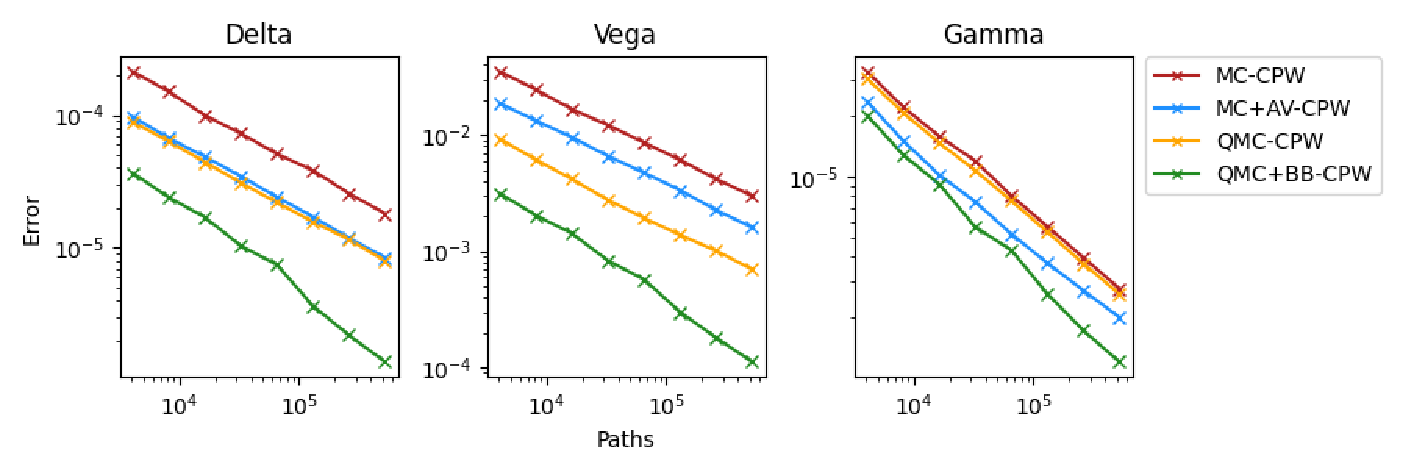
\includegraphics[width=1\textwidth]{figures/arithmetic path errors k=90.pdf}
    \caption{Errors in Greek estimates of an arithmetic Asian option with $S(0)=100$, $K=90$, $\sigma = 0.2$, $r=0.1$, $N=256$, and $T=1$ over $2^{12}$ to $2^{19}$ paths.}
    \label{fig:ArithmeticPathErrorsK90}
\end{figure}

\begin{figure}[H]
    \centering
    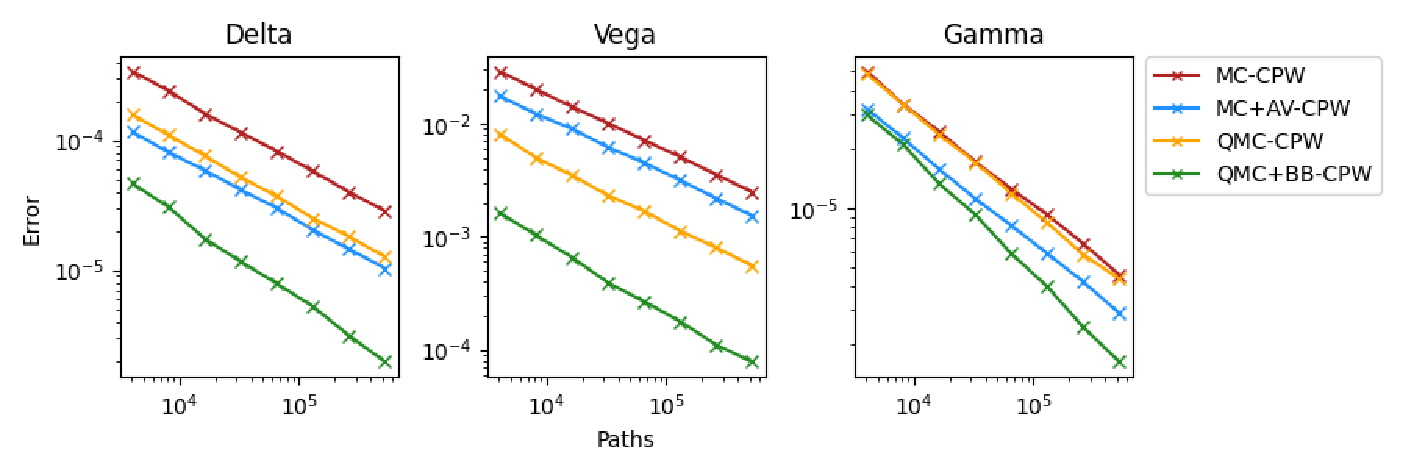
\includegraphics[width=1\textwidth]{figures/arithmetic path errors k=100.pdf}
    \caption{Errors in Greek estimates of an arithmetic Asian option with $S(0)=100$, $K=100$, $\sigma = 0.2$, $r=0.1$, $N=256$, and $T=1$ over $2^{12}$ to $2^{19}$ paths.}
    \label{fig:ArithmeticPathErrorsK100}
\end{figure}

\begin{figure}[H]
    \centering
    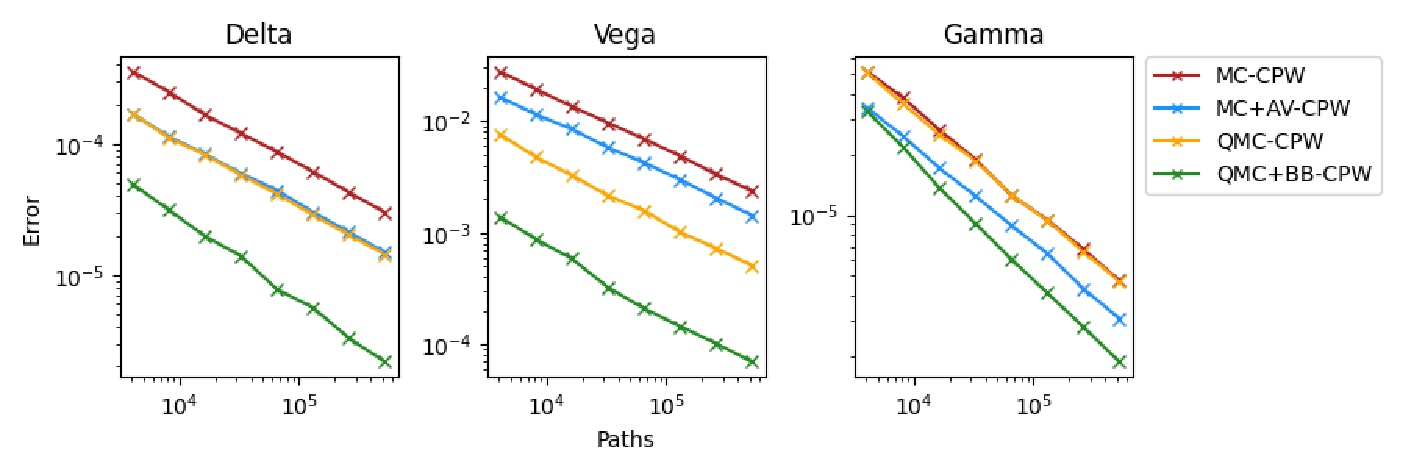
\includegraphics[width=1\textwidth]{figures/arithmetic path errors k=110.pdf}
    \caption{Errors in Greek estimates of an arithmetic Asian option with $S(0)=100$, $K=110$, $\sigma = 0.2$, $r=0.1$, $N=256$, and $T=1$ over $2^{12}$ to $2^{19}$ paths.}
    \label{fig:ArithmeticPathErrorsK110}
\end{figure}

\begin{itemize}
    \item For the arithmetic Asian estimates (figures \ref{fig:ArithmeticPathErrorsK90}-\ref{fig:ArithmeticPathErrorsK110}), QMC+BB-CPW is the best performing method across all number of paths and Greeks.
    \item For gamma estimates in figures \ref{fig:ArithmeticPathErrorsK90}-\ref{fig:ArithmeticPathErrorsK110} the advantage appears to increase as the number of paths increase.
    \item QMC-CPW is greatly outperformed by MC+AV-CPW for the arithmetic option's (figures \ref{fig:ArithmeticPathErrorsK90}-\ref{fig:ArithmeticPathErrorsK110}) gamma estimates of the arithmetic option whilst they perform similarly for delta.
    \item For the first order Greeks (delta and vega in figures \ref{fig:ArithmeticPathErrorsK90}-\ref{fig:ArithmeticPathErrorsK110}) QMC+BB-CPW has a large advantage over the other methods even at a small number of paths. However, for the second order Greek of gamma it's error is roughly equal to that of MC+AV-CPW at a small number of paths and it only gains a noticeable advantage as the number of paths increases.
\end{itemize}

\begin{figure}[H]
    \centering
    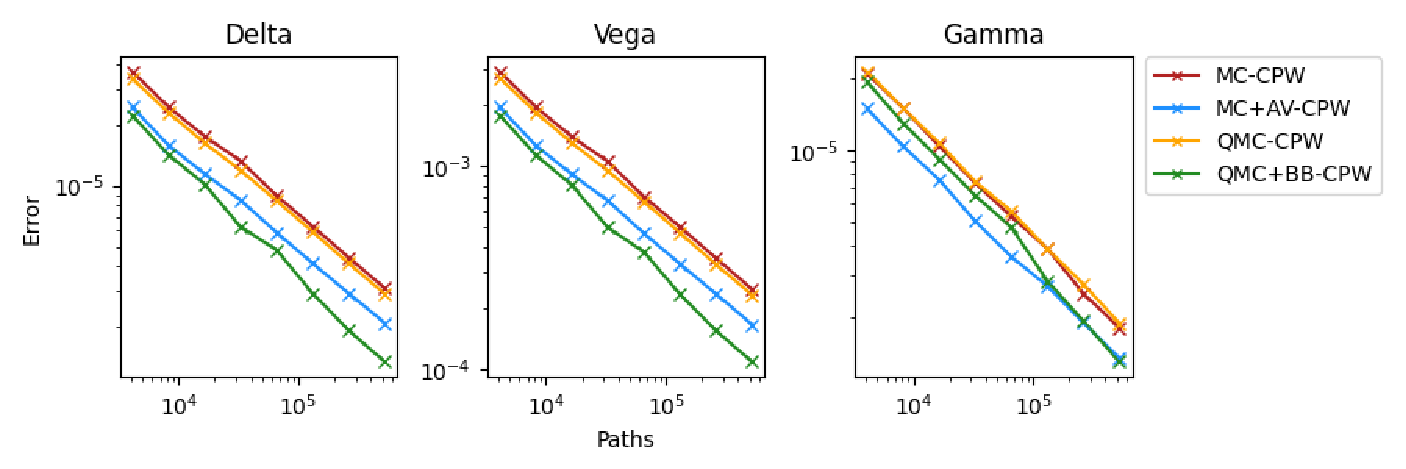
\includegraphics[width=1\textwidth]{figures/binary path errors k=90.pdf}
    \caption{Errors in Greek estimates of a binary Asian option with $S(0)=100$, $K=90$, $\sigma = 0.2$, $r=0.1$, $N=256$, and $T=1$ over $2^{12}$ to $2^{19}$ paths.}
    \label{fig:BinaryPathErrorsK90}
\end{figure}

\begin{figure}[H]
    \centering
    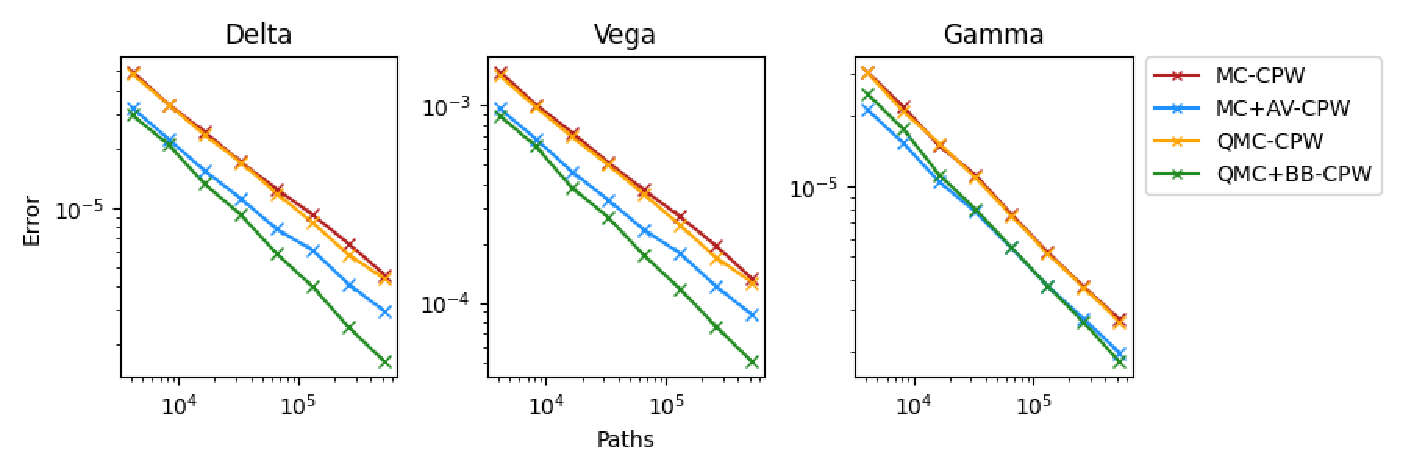
\includegraphics[width=1\textwidth]{figures/binary path errors k=100.pdf}
    \caption{Errors in Greek estimates of a binary Asian option with $S(0)=100$, $K=100$, $\sigma = 0.2$, $r=0.1$, $N=256$, and $T=1$ over $2^{12}$ to $2^{19}$ paths.}
    \label{fig:BinaryPathErrorsK100}
\end{figure}

\begin{figure}[H]
    \centering
    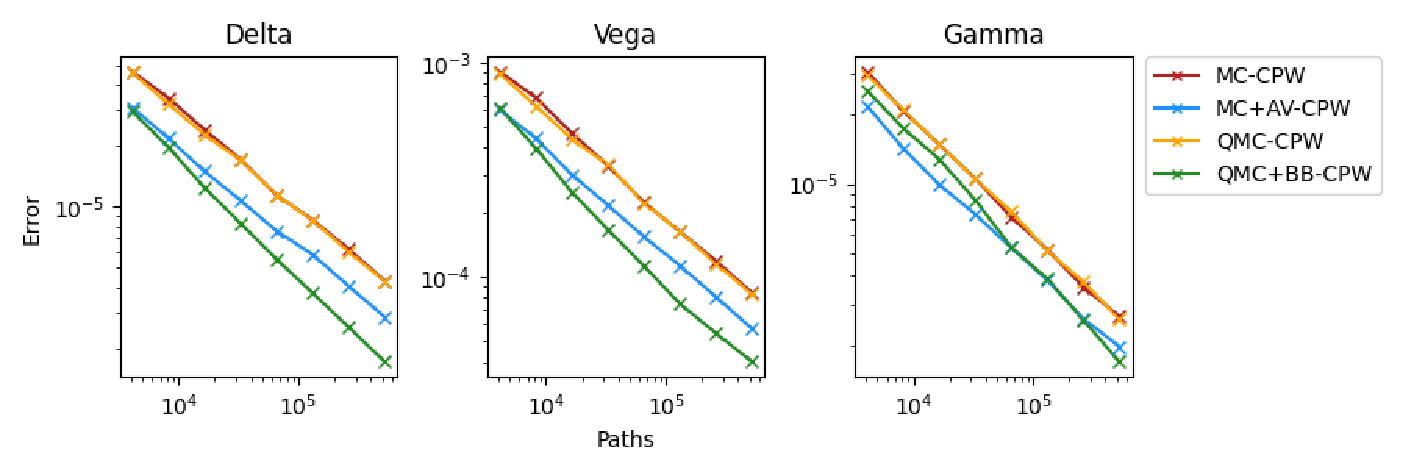
\includegraphics[width=1\textwidth]{figures/binary path errors k=110.pdf}
    \caption{Errors in Greek estimates of a binary Asian option with $S(0)=100$, $K=110$, $\sigma = 0.2$, $r=0.1$, $N=256$, and $T=1$ over $2^{12}$ to $2^{19}$ paths.}
    \label{fig:BinaryPathErrorsK110}
\end{figure}

\begin{itemize}
    \item The errors in the estimates for the binary Asian option (figures \ref{fig:BinaryPathErrorsK90}-\ref{fig:BinaryPathErrorsK110}) are much closer than that of the arithmetic Asian.
    \item For delta and vega of the binary option in figures \ref{fig:BinaryPathErrorsK90}-\ref{fig:BinaryPathErrorsK110}, QMC+BB-CPW is the superior method across all number paths.
    \item MC+AV-CPW tends to match and often outperform QMC+BB-CPW when the number of paths is smaller for the binary option (figures \ref{fig:BinaryPathErrorsK90}-\ref{fig:BinaryPathErrorsK110}). In fact, we only see MC+AV-CPW outperformed for gamma at a very high path number ($2^{19}$).
    \item For all estimates of the binary option (figures \ref{fig:BinaryPathErrorsK90}-\ref{fig:BinaryPathErrorsK110}) we see almost no improvement with QMC-CPW over MC-CPW.
\end{itemize}

\begin{figure}[H]
    \centering
    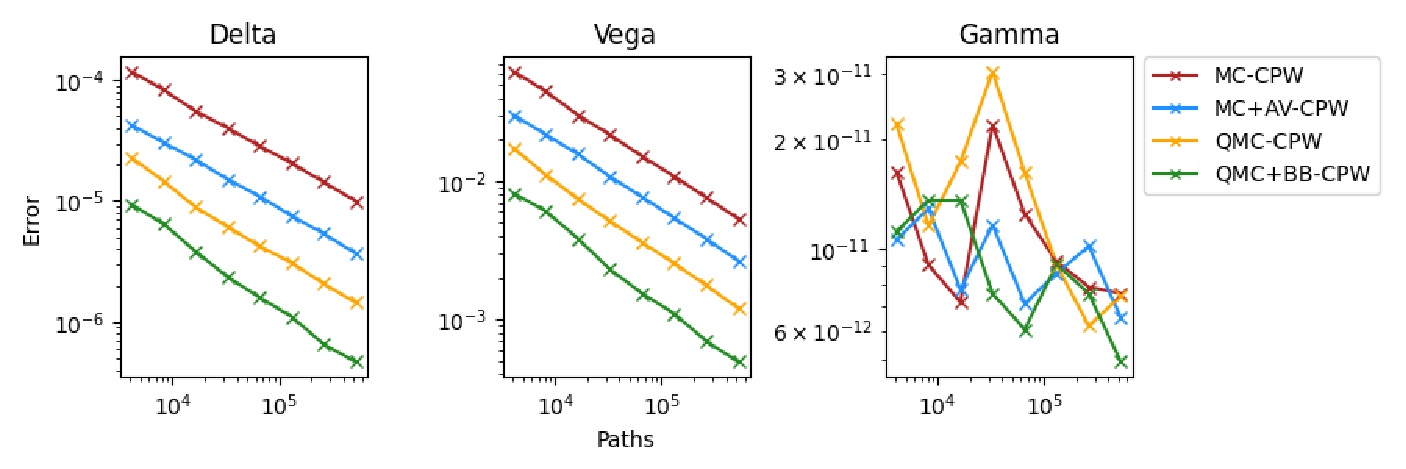
\includegraphics[width=1\textwidth]{figures/lookback path errors k=90.pdf}
    \caption{Errors in Greek estimates of a lookback option with $S(0)=100$, $K=90$, $\sigma = 0.2$, $r=0.1$, $N=256$, and $T=1$ over $2^{12}$ to $2^{19}$ paths.}
    \label{fig:LookbackPathErrorsK90}
\end{figure}

\begin{figure}[H]
    \centering
    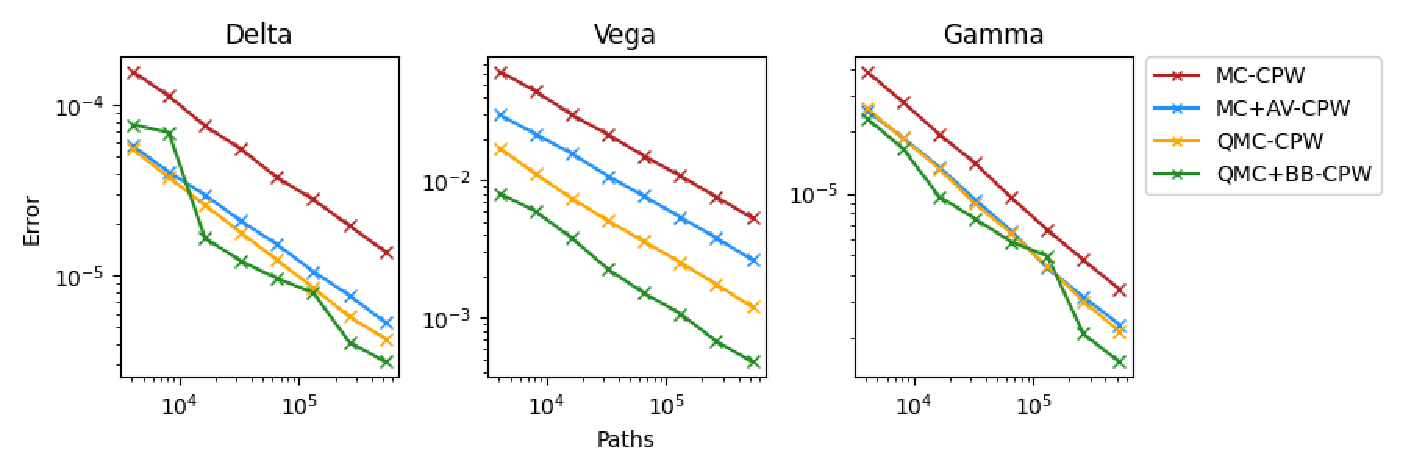
\includegraphics[width=1\textwidth]{figures/lookback path errors k=100.pdf}
    \caption{Errors in Greek estimates of a lookback option with $S(0)=100$, $K=100$, $\sigma = 0.2$, $r=0.1$, $N=256$, and $T=1$ over $2^{12}$ to $2^{19}$ paths.}
    \label{fig:LookbackPathErrorsK100}
\end{figure}

\begin{figure}[H]
    \centering
    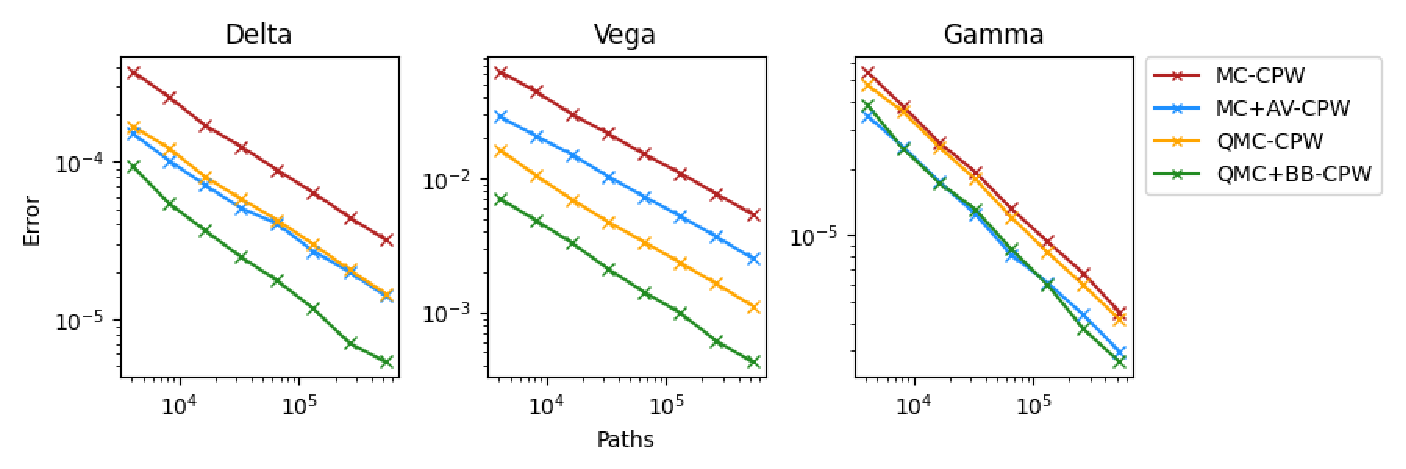
\includegraphics[width=1\textwidth]{figures/lookback path errors k=110.pdf}
    \caption{Errors in Greek estimates of a lookback option with $S(0)=100$, $K=110$, $\sigma = 0.2$, $r=0.1$, $N=256$, and $T=1$ over $2^{12}$ to $2^{19}$ paths.}
    \label{fig:LookbackPathErrorsK110}
\end{figure}

\begin{itemize}
    \item We see the largest variation in performance across the lookback estimates (figures \ref{fig:LookbackPathErrorsK90}-\ref{fig:LookbackPathErrorsK110}).
    \item For the gamma estimates when $K=90$ (in the money, figure \ref{fig:LookbackPathErrorsK90}) the errors are extremely small and don't follow the same monotonically decreasing trend we see in most other graphs.
    \item The vega estimates in figures \ref{fig:LookbackPathErrorsK90}-\ref{fig:LookbackPathErrorsK110} are the most consistent where we see MC-CPW, MC+AV-CPW, QMC-CPW, QMC+BB-CPW as the order from largest error to smallest for $K=90,100,110$.
    \item When the option is at the money in figure \ref{fig:LookbackPathErrorsK100}, we see the least improvement of QMC+BB-CPW over QMC-CPW when compared to other options and estimates, where it is outperformed at a smaller number of paths and even matched at $2^{17}$ paths.
\end{itemize}
 

The final objective was to achieve a significant speed up over a CPU implementation. For the three methods where we do not store the path, we see speedups for a single kernel run when compared to the naive sequential CPU implementation upwards of $500$x for those experiments with $64$ timesteps per path, and upwards of $900$x for those with $256$ timesteps.

The overhead of accessing global memory on device becomes apparent when we see the difference in the speedup between the QMC+BB-CPW experiments and the other methods. Due to having to store the Brownian bridge path construction and then repeatedly accessing the array in global memory we see a significant decrease in speedups from the previously mentioned values to around $200$x for both $64$ and $256$ timesteps. It is interesting to note that the lookback option sees the greatest speed improvement over the CPU.

Although tables \ref{tbl:vrfs-arithmetic}-\ref{tbl:vrfs-lookback} show that MC+AV-CPW outperforms QMC+BB-CPW in some instances, from figures \ref{fig:ArithmeticPathErrorsK90}-\ref{fig:LookbackPathErrorsK110} we see that as the number of paths increases past $2^{15}$, which is the value used for the tables, QMC+BB-CPW tends to become the best performing method.